
%% bare_conf.tex
%% V1.4b
%% 2015/08/26
%% by Michael Shell
%% See:
%% http://www.michaelshell.org/
%% for current contact information.
%%
%% This is a skeleton file demonstrating the use of IEEEtran.cls
%% (requires IEEEtran.cls version 1.8b or later) with an IEEE
%% conference paper.
%%
%% Support sites:
%% http://www.michaelshell.org/tex/ieeetran/
%% http://www.ctan.org/pkg/ieeetran
%% and
%% http://www.ieee.org/
%%*************************************************************************
%% Legal Notice:
%% This code is offered as-is without any warranty either expressed or
%% implied; without even the implied warranty of MERCHANTABILITY or
%% FITNESS FOR A PARTICULAR PURPOSE!
%% User assumes all risk.
%% In no event shall the IEEE or any contributor to this code be liable for
%% any damages or losses, including, but not limited to, incidental,
%% consequential, or any other damages, resulting from the use or misuse
%% of any information contained here.
%%
%% All comments are the opinions of their respective authors and are not
%% necessarily endorsed by the IEEE.
%%
%% This work is distributed under the LaTeX Project Public License (LPPL)
%% ( http://www.latex-project.org/ ) version 1.3, and may be freely used,
%% distributed and modified. A copy of the LPPL, version 1.3, is included
%% in the base LaTeX documentation of all distributions of LaTeX released
%% 2003/12/01 or later.
%% Retain all contribution notices and credits.
%% ** Modified files should be clearly indicated as such, including  **
%% ** renaming them and changing author support contact information. **
%%*************************************************************************



\documentclass[a4paper,conference]{IEEEtran}

\def\citepunt{,}

\usepackage[pdftex]{graphicx}
\ifCLASSOPTIONcompsoc
  \usepackage[caption=false,font=normalsize,labelfont=sf,textfont=sf]{subfig}
\else
  \usepackage[caption=false,font=footnotesize]{subfig}
\fi
\usepackage{comment}
\usepackage{float}
\usepackage{mathtools}
\usepackage{amsfonts}
\usepackage{bm}
\usepackage{pgf,tikz,pgfplots}
\usetikzlibrary{calc}

\DeclarePairedDelimiter\ceil{\lceil}{\rceil}
\DeclarePairedDelimiter\floor{\lfloor}{\rfloor}

\DeclareMathOperator{\vect}{vec}

\newcommand{\R}{\mathbb{R}}
\newcommand{\A}{\mathcal{A}}
\newcommand{\D}{\mathcal{D}}
\newcommand{\I}{\hat{I}}
\newcommand{\Z}{\mathbb{Z}}
\newcommand{\m}[1]{{\mathrm{\bf #1}}}
\newcommand{\E}{\tilde{\m{I}}}
\newcommand{\F}{\hat{F}}
\newcommand{\lI}{\m{I}}
\newcommand{\mF}{\m{F}}
\newcommand{\bF}{\mathcal{F}}
\newcommand{\J}{\hat{J}}
\newcommand{\lJ}{\m{J}}
\newcommand{\pD}{D^\prime}
\newcommand{\eF}{\hat{\mF}}
\newcommand{\gN}{\m{N}}
\newcommand{\W}{\m{W}}
\newcommand{\M}{\mathcal{M}}
\newcommand{\Pa}{\mathcal{P}}
\newcommand{\pDD}{\D^\prime}

\definecolor{navy}{RGB}{0,0,137}
\definecolor{tealDeer}{RGB}{148,232,180}
\definecolor{dodgerBlue}{RGB}{18,161,255}
\definecolor{citrine}{RGB}{230, 194, 8}
\definecolor{violet}{RGB}{112,5,164}
\definecolor{navyPurple}{RGB}{172,86,253}
\definecolor{heliotrope}{RGB}{236,93,253}

% correct bad hyphenation here
\hyphenation{op-tical net-works semi-conduc-tor}


\begin{document}

\title{Learning CNN filters from user-drawn image makers for coconut-tree image classification}

% make the title area
\maketitle

\begin{abstract}
 Identifying species of trees in aerial images is essential for land-use classification, plantation monitoring, and impact assessment of natural disasters. The manual identification of trees in aerial images is tedious, costly, and error-prone, so automatic classification methods are necessary. Convolutional Neural Network (CNN) models have well succeeded in image classification applications from different domains. However, CNN models usually require intensive manual annotation to create large training sets. A CNN may be conceptually divided into convolutional layers for feature extraction and fully connected layers for classification. We present a method that needs a minimal set of user-selected images to train the CNN's feature extractor, considerably reducing the number of images to train its classifier. The method learns the filters of each convolutional layer from user-drawn markers in image regions that discriminate classes, allowing direct human expert interference in the training process. It does not rely on optimization based on backpropagation, which considerably reduces the number of required images. We demonstrate its advantages on binary classification of coconut-tree images against a popular CNN model.
\end{abstract}

\section{Introduction}
Deep learning has proven to be applicable to different tasks, from image classification to data synthesis \cite{goodfellow2016deep}. In remote sensing, the applications have involved segmentation of terrain images \cite{kemker2018algorithms, kampffmeyer2016semantic, hamaguchi2018effective}, building identification \cite{xu2018building, lu2018detecting, liu2018multilevel}, and deforestation monitoring \cite{bragilevsky2017deep}. In this work, we are interested in 
 identifying species of trees from aerial images. The topic is important for land-use classification, plantation monitoring, and damage assessment of natural disasters. As the plantations can span very large areas, the manual identification of each tree is costly, tedious, and error-prone, and so automatic classification methods are necessary. 

Classification of tree species in aerial images has been actively investigated~\cite{fassnacht2016review}. In \cite{puttemans2018comparing} and~\cite{aparna2018cnn}, the authors present automatic solutions to detect coconut trees based on convolutional neural network (CNN) models. Despite these recent advances, CNN models usually require considerable human effort in image annotation to create large training sets. Vargas-Muñoz et al.~\cite{8899005} propose an approach to mitigate the problem based on active learning. The method explores data projection techniques to allow simultaneous annotation of multiple patches as having or not a coconut tree. It then uses a CNN to identify the candidate patches with a coconut tree. We adopt another alternative in this work -- the design of simplified CNN models from reduced annotated image sets and assistance of a human expert. 

The design of CNN models without a human expert as part of the training loop leaves several questions unanswered: (1) How to choose the most reasonable model, with acceptable effectiveness, and as simple as needed for a given classification problem? (2) How to train that model from a reduced number of images?  (3) Can the user explain the decisions of that model? (4) Can that model improve from human corrections? The first question requires to explore human knowledge about the classification technique and the problem of interest. The second one requires to reduce as much as possible the human effort to train a CNN model. The third issue is related to human understanding. It may explore data visualization techniques to explain the model's decisions and guide human decisions concerning the design of the model. The fourth question is also essential during training, and it is related to human control over the process. They all lead to the importance of involving human experts (users) during the machine learning process.

In this paper, we present significant advances related to the questions (1) and (2). First, we conceptually divide a CNN into convolutional layers for feature extraction and fully connected layers for feature space reduction and classification. Each convolutional layer contains a filter bank, an activation function, and alternative operations (e.g., pooling, batch normalization).  As the number of convolutional layers increases (deeper is the model), higher is the number of annotated samples required to train the model by backpropagation. 

We present a method that needs a minimal set of images to learn the filters of each convolutional layer. The user selects the number of convolutional layers, a few training images, and draws markers in regions that best discriminate the classes. We explain how the classes may appear in distinct clusters of a local feature space defined by patches as extracted from marker pixels at the input of each convolutional layer. Patch size (number of weights per filter) is also a user choice. The architecture of the network can be optimized by observing its results on a small validation set or based on data visualization techniques~\cite{rauber2016visualizing}. The method uses clustering and defines the weights of the filters from the centroids of the clusters. Such filters must activate the discriminant regions in the output of the given convolutional layer, and the process repeats in a layer-by-layer fashion with usually no need for new markers. 

We demonstrate the advantages of this new technique on binary image classification of coconut-tree images against a popular CNN model, VGG-16~\cite{simonyan2014very}. First, the user can directly interfere and verify the markers' effectiveness in the training process.  The strategy allows user control and a better understanding of CNN models. Second, very few images per class (e.g., less than five) are usually enough. Third, by eliminating the need for optimization of convolutional layers by backpropagation, the method can considerably reduce the number of annotated images to train the fully connected layers.  Fourth, the technique is application-independent, and so it might be useful in other image classification problems. 




\section{Learning filters from markers}
\label{sec:method}

Convolutional neural networks perform well in image classification tasks due to its capability of extracting features. That is, convolutional layers produce great descriptors that can be used by the classifier. Conventionally, during the training process, an algorithm tries to minimize a loss function that measures how good the classifier is performing with the features given by the feature extractor. The algorithm of optimization tries through backpropagation to find out which features to extract. Our method is based on the idea that the network designer is an expert in the application domain or knows well enough to indicate which are the relevant characteristics of the objects of interest. Hence, it does not rely on the optimization of some loss function to learn filters for those relevant characteristics. In our approach, the network designer highlights features that she believes are the ones that characterize each class by placing markers. Those markers are used to learn the filters to identify the features they represent.

Let $\D$ be a dataset of images, and let $I \in \D$ be an image with dimensions $X \times Y$. A marker $m$ is associated with a pixel $p(m) = (x, y)$ and has a label $L(m) = c$. Let $M(I)$ be the set of markers of image $I$.  For each maker $m \in M(I)$, we create a patch $P$ with dimensions $k \times k$ from a window centered in the marker's pixel as $P(I, x ,y) = I(x+i, y+j)$ for $i, j = -\floor{k/2}, \ldots, \floor{k/2}$.We pad images with $0$ so that we can create patches from border pixels. For each class, we create a set of patches made using the markers of that class. Let \[\mathcal{P}_c = \bigcup_{ I \in \D, m \in M(I) :\, L(m) = c}{P(I, p(m))}\] be the set of all patches made from markers of class $c$.

Given set of patches $\Pa_c$, we can use a clustering algorithm to discover groups in $\Pa_c$. Each group represents local patterns of class $c$, highlighted by the designer through the markers. Since the centroid of each cluster must be a good representative of the characteristics of the group, we can use them as filters to enhance those patterns in the images of $\D$. We must do this for each class.

However, for it to work properly, patches and images need to be centered at the origin. For this, we use the information from the patches of all classes to calculate the mean and standard deviation per band. If the patches are representative of images in $\D$, the mean and standard deviation per band of $\Pa$ are close to the mean and standard deviation per band in $\D$.

\begin{comment}
\begin{figure}[t]
  \begin{center}
     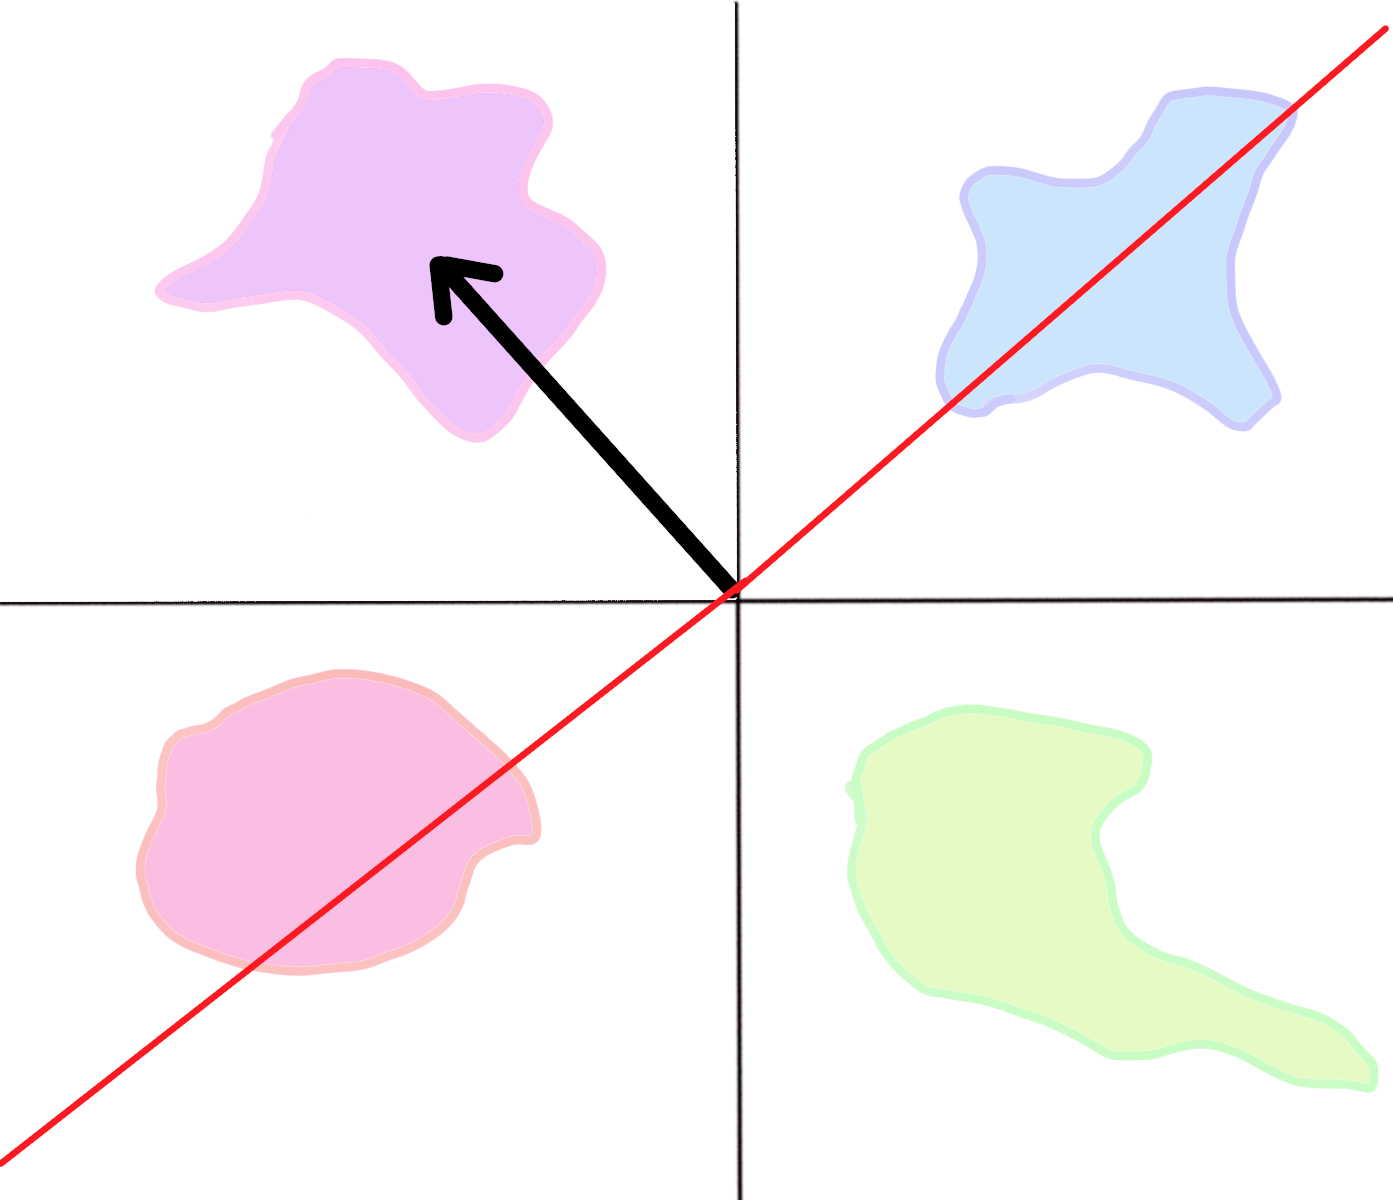
\includegraphics[width=0.8\linewidth]{figures/filter.png}
  \end{center}
  \caption{Filter learned from clustering.}
  \label{fig:filter}
\end{figure}
\end{comment}


Let $F$ be a filter with dimension $k \times k$, and let $\pi$ be the patch around pixel $(x,y)$ also with dimension $k \times k$. By the definition of convolution in deep learning, we can interpret this operation for a pixel $(x, y)$ as the dot product between the kernel vector $\vect(F)$ and the vector of a patch $\vect(\pi)$ around this pixel, that is, the convolution in $(x, y)$ is the same as $\vect(F) \cdot \vect(\pi)$. Thus, let $H$ be a hyperplane orthogonal to vector $\vect(F)$. Vectors similar to $\vect(F)$ must fall on the same side of the hyperplane as $\vect(F)$. Therefore, if vector $\vect(\pi)$ is on the same side of $H$ as $\vect(F)$, then the dot product between $\vect(\pi)$ and $\vect(F)$ is positive, and it is negative otherwise. Thus, the dot product between the centroid of a cluster and each of the vectors of that cluster must be positive, which implies that the centroid is a good filter to identify the pattern described by that cluster. Hence, if we throw away the negative values, applying convolution with centroids as filters must highlight regions with a certain pattern that the network designer believes is important.

Since all patches used to produce the filters are centered around the origin, as well as the images of $\D$, we have that the hyperplanes orthogonal to the filters contain the origin. Therefore, there is no need for bias.

Each convolutional layer is trained individually, one layer at a time. After the convolution operation, we apply the ReLU function to eliminate negative activations and the max pooling operation to aggregate local information. We preserve the convolutional layers' output dimensions so that we can use the same markers used in the previous layer. The new patches are generated from the previous convolutional layer output, and the whole process is repeated to find the filters of the next one.

\begin{figure}[!t]
  \centering
  \subfloat[\label{fig:ex-groups}]
  {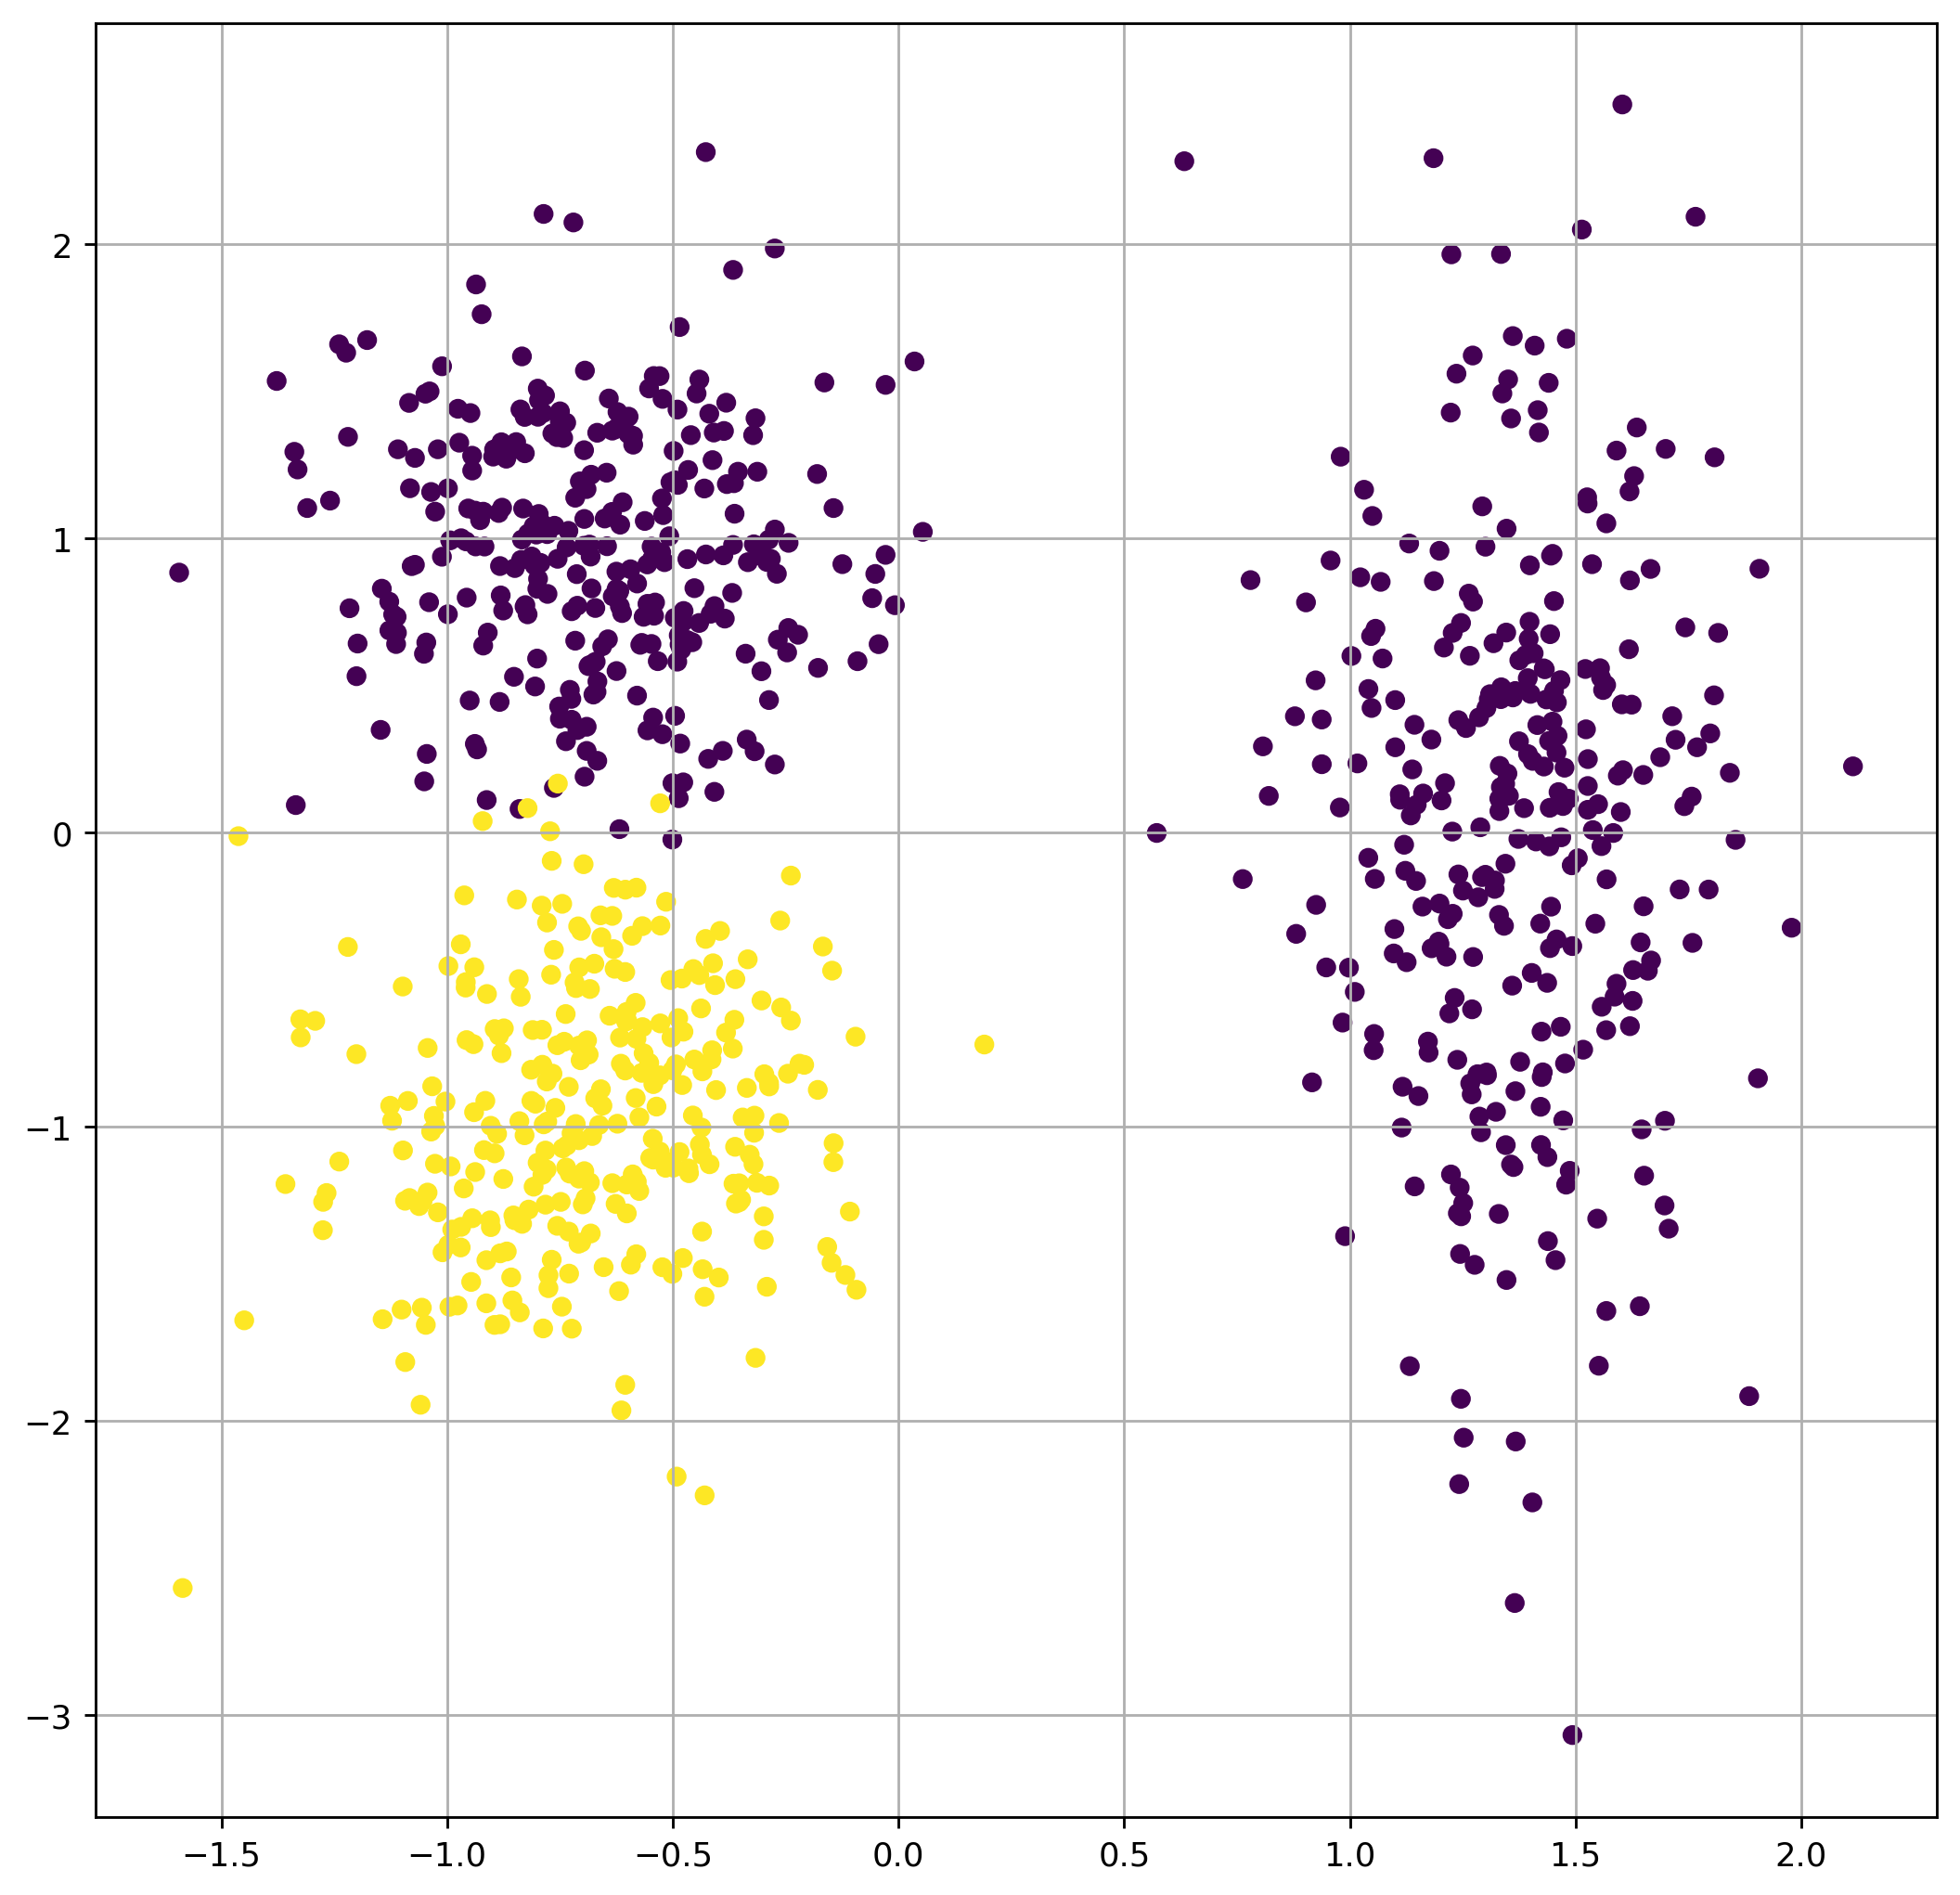
\includegraphics[width=.35\linewidth]{figures/example_groups/groups_centered}}
  ~
  \subfloat[\label{fig:ex-groups-after}]{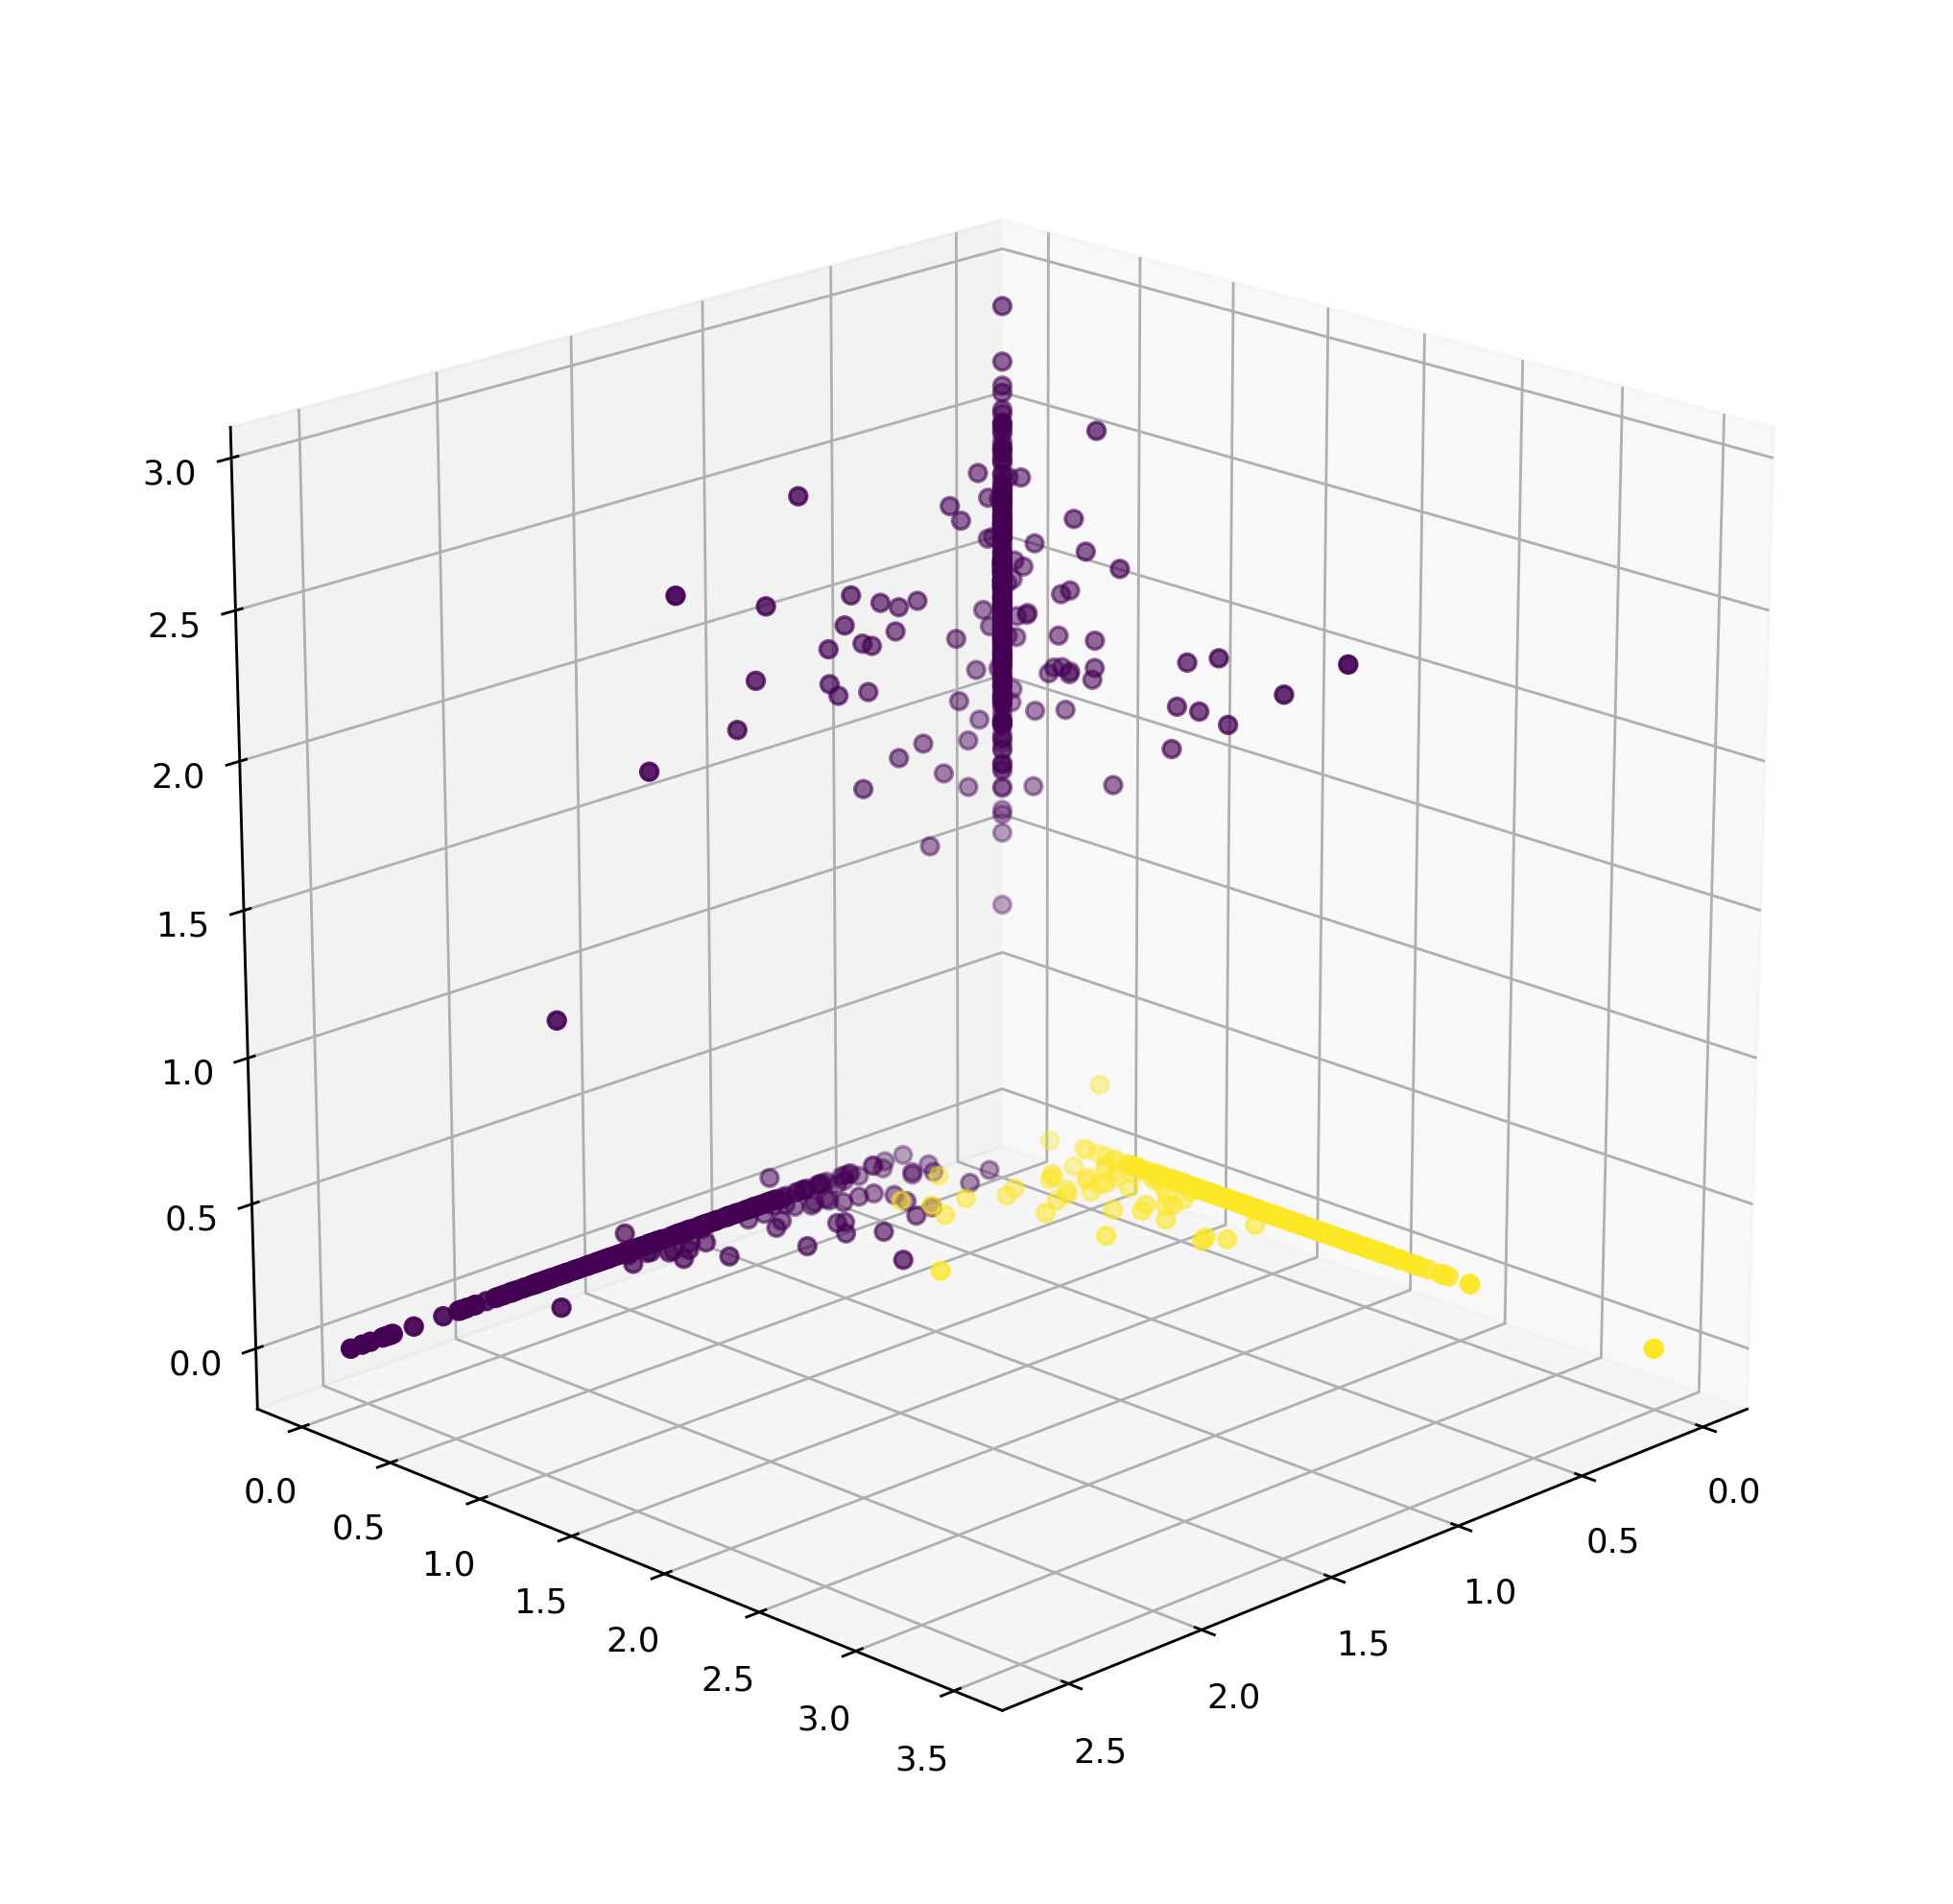
\includegraphics[width=.45\linewidth]{figures/example_groups/groups3d_centered}
  }
  \caption{Example of application of convolution with groups centers as filters' weights: (a) Groups of three classes centered on the origin; (b) Groups after applying convolution and activation operations. }
  \label{fig:filter}
\end{figure}

\begin{figure}
  \begin{center}
  \tikzset{
    treenode/.style = {shape=rectangle, rounded corners,
                       draw=black, align=center, line width=width},
    specialedge/.style = {line width=1.5pt}
  }

  \begin{tikzpicture}
    [
      grow                    = down,
      sibling distance        = 5em,
      level distance          = 3em,
      edge from parent/.style = {draw=black},
      every node/.style       = {treenode},
      sloped
    ]
    \node [treenode, fill=tealDeer, label = {[label distance = 0.5em]}] (v0) {Conv$(60 \times 7 \times 7)$}
      child {
        child {
          child {
                child {
                  node [treenode, fill=navyPurple] {Classifier}
                  edge from parent
                }
                node [treenode, fill=tealDeer] {BatchNorm}
                edge from parent
           }
          node [treenode, fill=tealDeer] {MaxPool$(3\times3)$}
          edge from parent
        }
        node [treenode, fill=tealDeer, label = {[label distance = 0.5em] }] {ReLU} 
        edge from parent
      };

  \end{tikzpicture}
  \end{center}
  \label{fig:tree}
\end{figure}

To exemplify our method, we create a synthetic dataset of points of two classes. We can see this dataset in Figure \ref{fig:ex-groups}. The points are distributed in two regions, and it is not possible to separate the yellow class linearly from the violet class. To center the points,  we subtracted the mean and divided by the standard deviation. If we look only to violet points, it is clear that they form two clusters. In turn, the yellow dots form a single cluster. We then take the center of each of these three clusters and apply convolution to the set of points using these centers as filters. The result of the convolution after applying the ReLU function can be seen in Figure \ref{fig:ex-groups-after}. For most points after the transformation made by convolution and the ReLU function, only one coordinate was positive, this being the coordinate which value is the internal product with the center of the cluster of which these points are part. These points lie along the three axes of space $\mathbb{R}^3$, each cluster on an axis. The other points are farthest from their cluster center, and the internal product with the center of another cluster is also positive. Cluster centers functioned as good filters to detect similar points, even though they detected points from other clusters.

\section{Experiments}
We use a dataset formed from patches of aerial images made by \cite{8899005} from imagery provided by WeRobotics. The imagery with a resolution of 8cm was captured by the World Bank's UAVs for Disaster Resilience Program, collaborating with WeRobotics and OpenAerialMap in the Kingdom of Tonga in October 2017. The Humanitarian OpenStreetMap community provided the annotation. The dataset consists of 13587 patches of dimensions $90 \times 90$ of coconut (10268) and non-coconut (3319). The latter class has a large variability. The problem of interest is to classify the images in one of the two classes. We only report experiments with one dataset due to the space limitation.

As in reality, labeling images is a costly and time-consuming process, and then we assume that we only knew the correct labels of a small set of samples (one hundred images for each class, totaling two hundred images). That way, we would have only those two hundred images to train any models that we would use to try to solve the problem.

To reduce the impact of chance on the results, we randomly selected three sets of 200 images for training and three sets of 11387 images for testing. We wanted to represent a scenario where the network designer did not have much effort to annotate all these images. From each of these sets of training images, we selected four images using the 2D space projection of the 200 images using the t-SNE. We tried to select images that were part of more cohesive groups. Thus, these images are more likely to have characteristics that represent their group.

\begin{figure}[!t]
    \centering
    \subfloat[\label{fig:markers1}]{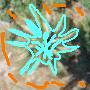
\includegraphics[width=.3\linewidth]{figures/markers1}
    }
    ~
    \subfloat[\label{fig:markers2}]{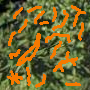
\includegraphics[width=.3\linewidth]{figures/markers2}
    }
    \\
    \subfloat[\label{fig:markers3}]{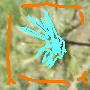
\includegraphics[width=.3\linewidth]{figures/markers3}
    }
    ~
    \subfloat[\label{fig:markers4}]{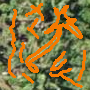
\includegraphics[width=.3\linewidth]{figures/markers4}
    }
    \caption{Markers used for training. (a) Markers on an image which contains a coconut tree. (b) Markers on an image which does not contain a coconut tree. (c) Markers on an image which does not contain a coconut tree. (d) Markers on an image which does not contain a coconut tree.}
    \label{fig:markers}
\end{figure}

We placed markers on these images in regions that we consider important to identify the coconut and non-coconut (more diverse) classes. In Figure \ref{fig:markers} we can the four images of one the splits. With the markers, we created a convolutional layer with filters of dimensions $7 \times 7$ using the method described in Section \ref{sec:method}. The network architecture can be seen in the Figure. We used a classifier similar to that of VGG-16. We used K-means to cluster the coconut tree patches in 30 clusters and the non-coconut tree patches in also 30 clusters to find the convolutional layer filter. 

\begin{table}[!t]
  \begin{center}
  \begin{tabular}{|l|c|c|c|}
  \hline
   Method & Precision & Recall & F-score \\
  \hline\hline
    I-Ours & $0.856 \pm 0.014$ & $0.836 \pm 0.020$ & $0.842 \pm 0.018$\\
    II-Ours (B) & $0.851 \pm 0.018$ & $0.834 \pm 0.023$ & $0.839 \pm 0.021$\\
    III-Ours (SVM) & $0.836 \pm 0.015 $ & $ 0.793 \pm 0.025$ & $ 0.804 \pm 0.022$\\
    IV-VGG & $0.84 \pm 0.01$ & $0.76 \pm 0.03$ & $0.77 \pm 0.02 $ \\
    V-VGG (PT) & $0.84 \pm 0.01$ & $0.75 \pm 0.03$ & $0.77 \pm 0.02 $ \\
  \hline
  \end{tabular}
  \end{center}
  \caption{Results.}
  \label{tab:results}
\end{table}


We tested three scenarios: (I) using out method to learn the feature extractor weights and the classifier with backpropagation; (II) using our method as initialization and train the whole model with backpropagation; (III) using SVM Linear as classification. For VGG-16, we tested two secenarios: (IV) initializing with Xavier initialization and training from screath; (V) using ImageNet weights and training with the training set images. The results can be seen in Table \ref{tab:results}. As the experiments were repeated three times, we reported the mean and standard deviation of each the metrics in the test set. 

\begin{figure}
  \centering
  \subfloat{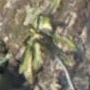
\includegraphics[width=.3\linewidth]{figures/qualitative/ours/upper-coco-108.png}
  }
  ~
  \subfloat{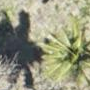
\includegraphics[width=.3\linewidth]{figures/qualitative/ours/upper-coco-2473.png}
  }
  ~
  \subfloat{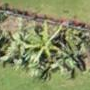
\includegraphics[width=.3\linewidth]{figures/qualitative/ours/upper-non_coco-506.png}
  }
  \\
  \subfloat{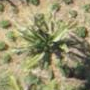
\includegraphics[width=.3\linewidth]{figures/qualitative/vgg/lower-coco-1098.png}
  }
  ~
  \subfloat{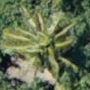
\includegraphics[width=.3\linewidth]{figures/qualitative/vgg/lower-coco-2400.png}
  }
  ~
  \subfloat{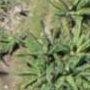
\includegraphics[width=.3\linewidth]{figures/qualitative/vgg/lower-non_coco-105.png}
  }
  \caption{Misclassified images. The first row has images misclassified by the network trained by our method, and the second row has images misclassified by VGG-16. The two first images of a row have coconut trees.}
  \label{fig:ex-classification}
\end{figure}

Our method achieved better precision than conventionally trained VGG, and the difference between precision and recall is much smaller. The Linear SVM did not prove to be a good classifier like the MLP, but, on average, it still got a little better than the VGG-16. Using our method as initialization and training the entire network with backpropagation did not improve the result; this implies that the filters we created are already good filters given the training set. Our feature extractor training method was able to learn good filters from a minimal set of images. VGG has many parameters to learn, so it is susceptible to overfitting with such a small training set. We do not use any technique to handle small data sets to train VGG because we intended to verify our approach viability, and these techniques could also be used with our method. In Figure \ref{fig:ex-classification} we can see examples of misclassified images. In these images, coconut trees appear in different angles, sizes, and shapes, or the boundaries between the coconut tree and the background are tenuous, making it more difficult to identify them. In turn, images that do not contain coconut trees, contain trees that resemble their shape. The network designer could put markers in those images in other to improve the feature extractor.

\begin{figure}
  \centering
  \subfloat[\label{fig:vis-input}]{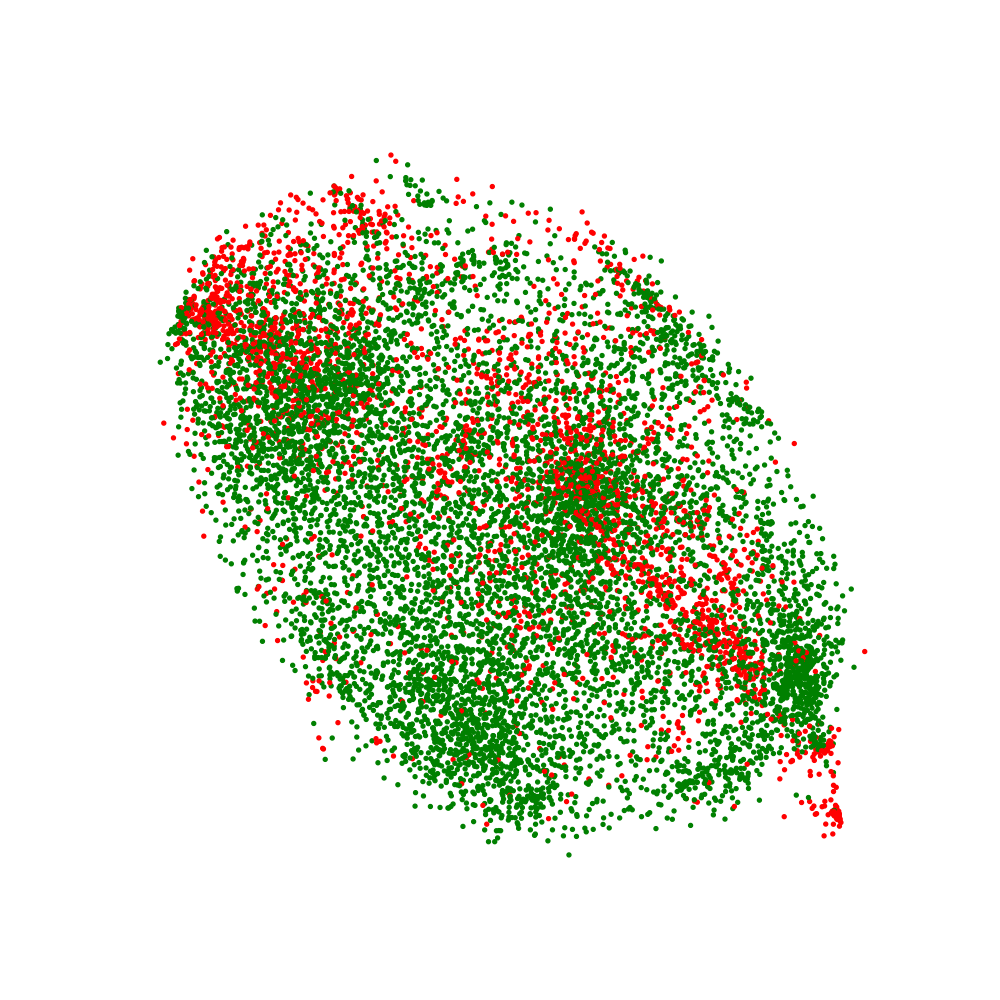
\includegraphics[width=.3\linewidth]{figures/input}
  }
  ~
  \subfloat[\label{fig:vis-feature-extractor}]{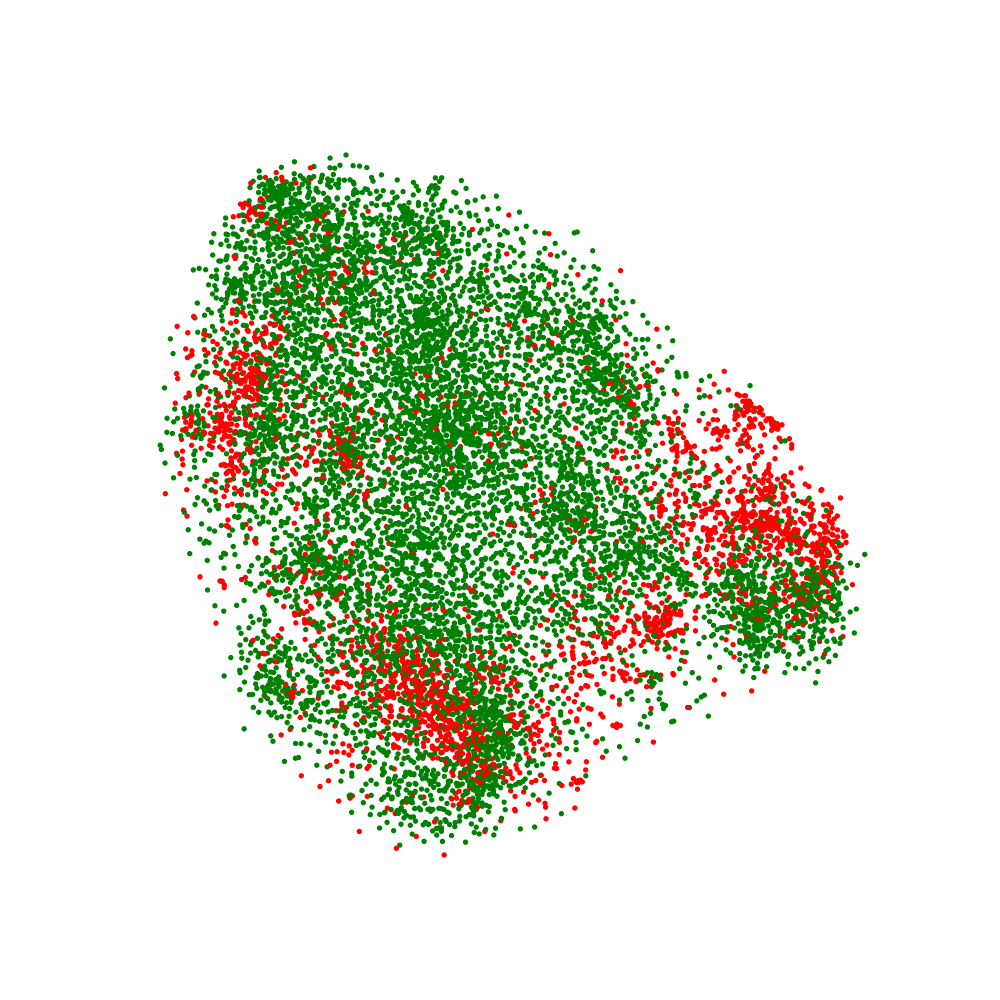
\includegraphics[width=.3\linewidth]{figures/feature_extractor}
  }
  ~
  \subfloat[]{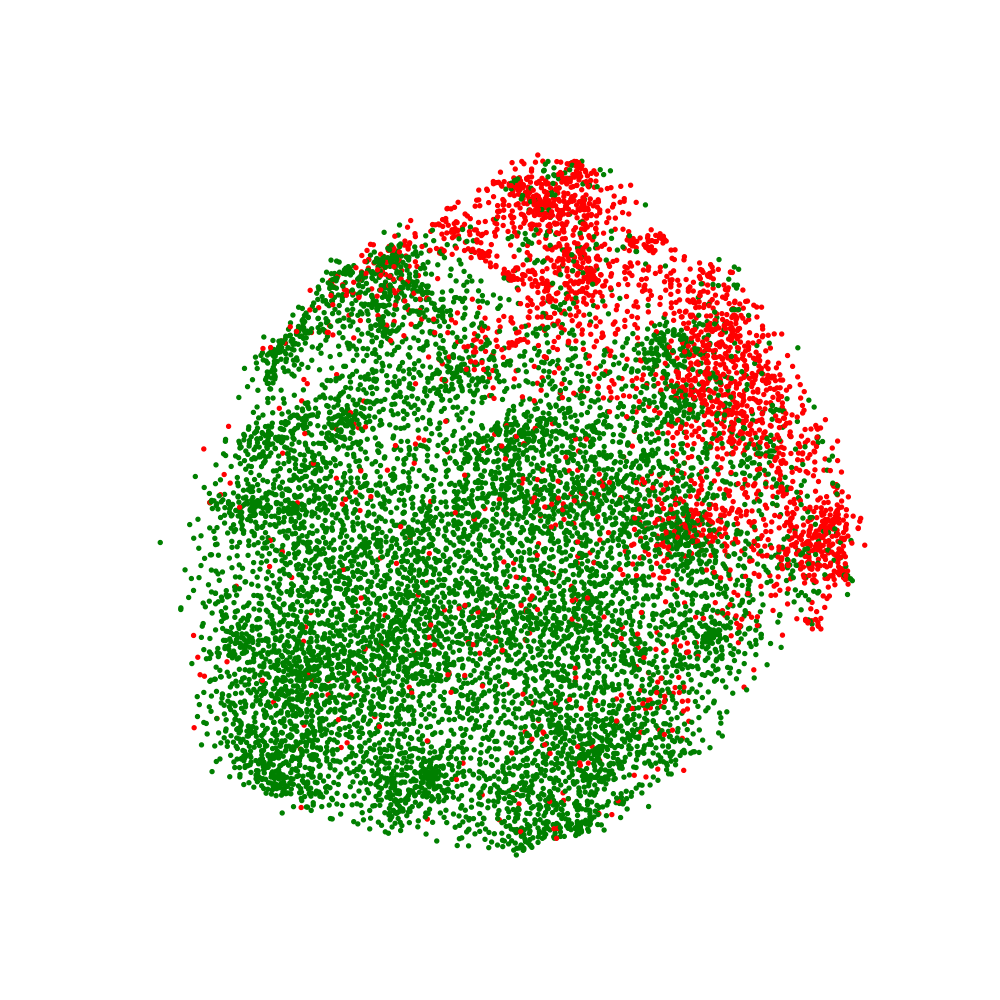
\includegraphics[width=.3\linewidth]{figures/classifier}
  \label{fig:vis-classifier}}
  \caption{This image shows visualizations of the input images and the intermediate layer's outputs. Red points represent background images, and green points represent images that have a coconut tree. The projection from high dimensionality space to 2D was made using t-SNE. The original image shows much overlap between the classes; after applying the feature extractor with only one convolutional layer, we can see that the overlapping decreases considerably. Before the decision layer, the last layer put most of the images from one class on one side and the other on the other side. (a) Visualization of original image feature space. (b) Visualization of the feature extractor's outputs. (c) Visualization of outputs from the last classifier hidden layer.}
\end{figure}

As motivated by Rauber et al. \cite{rauber2016visualizing}, we made projections of three stages of the network using t-SNE \cite{maaten2008visualizing} to understand how the feature extractor trained with our method transforms the image spaces. In Figure \ref{fig:vis-input}, we can see the projection of the original images (in the LAB color space). Red points are images that contain coconut trees, and green points are images that do not contain coconut trees. In the projection in the image of Figure \ref{fig:vis-input}, we see that the images of coconut trees and non-coconut trees are almost entirely overlapping. Coconut tree images are more frequent in some regions but are very dispersed. In the image of Figure \ref{fig:vis-feature-extractor}, we see the projection of the feature extractor output. The coconut tree images are more concentrated, forming some clusters, and it is possible to notice that there is much less overlap. Finally, we see in Figure \ref{fig:vis-classifier} the output of the previous layer of the decision layer of the classifier. The classifier managed to organize conquest and non-coconut images in different regions of space, although there is overlap as the model failed to achieve 100\% accuracy.

\section{Conclusions}

We present a way to train a feature extractor without using backpropagation capable of learning good filters from a minimal set of images. To evaluate the method, we proposed experiments to classify images that contain achievements. Our approach has achieved competitive results with state of the art.

\bibliographystyle{IEEEtran}
\bibliography{bibliography}

\end{document}


